\documentclass[tikz, margin=2mm]{standalone}
\usepackage{fontawesome}
\usepackage{sans}
\usepackage{tikz}
\usetikzlibrary{matrix, positioning,fit,backgrounds}


\begin{document}

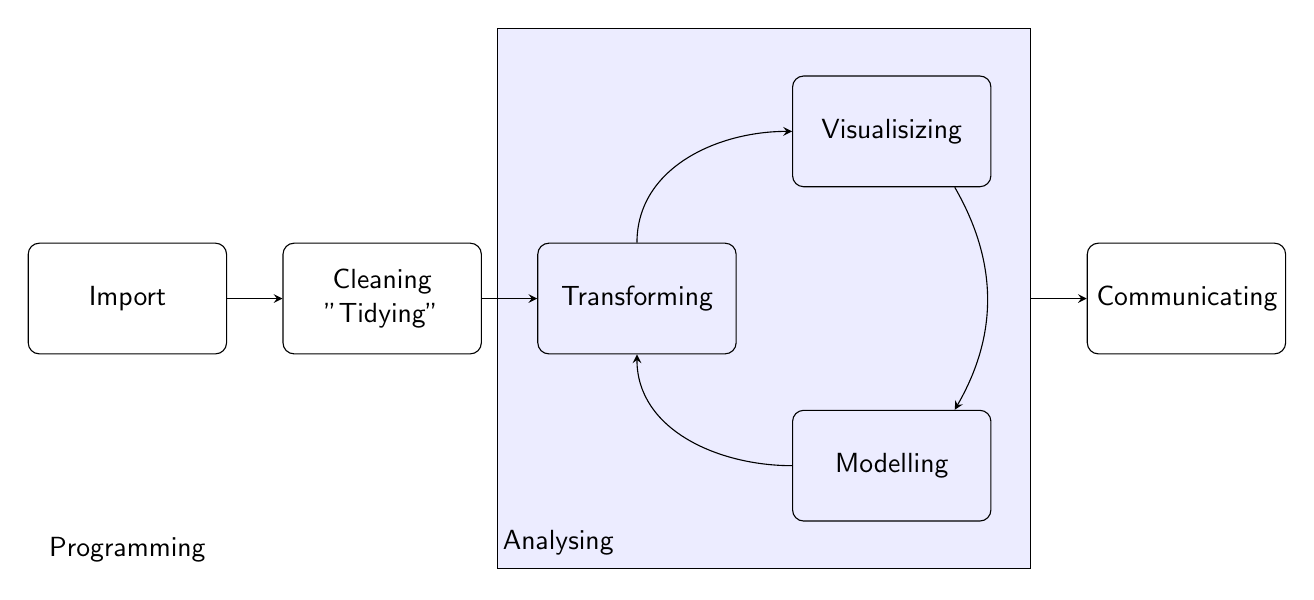
\begin{tikzpicture}[
	node distance=2em and 2em,
	block/.style={rectangle, draw, 
		text width=6.5em, text centered, rounded corners, minimum height=4em},
	line/.style={draw, -stealth},
	]
	\node[block] (imp) {Import};
	\node[below=of imp,yshift=-15mm] {Programming};
	\node[block,right= of imp] (tidy) {Cleaning\\"Tidying"};  
	\node[block,right= of tidy] (trans) {Transforming};  
	\node[block, above right= of trans] (viz) {Visualisizing};
	\node[block, below right= of trans] (mod) {Modelling};
	\begin{scope}[on background layer]
		\node[draw,fill=blue!15, fill opacity=0.5,inner xsep=5mm,inner  
		ysep=6mm,fit=(trans)(viz)(mod)](ana){}; %Alternative Füllnug top color=white,bottom color=blue!25
	\end{scope}
	\node[below=of trans,yshift=-14mm,xshift=-10mm] {Analysing};
	\node[block, right=of ana] (kom) {Communicating};

	%Verbindungspfeile		
	\path[line] (imp.east) to (tidy.west);
	\path[line] (tidy.east) to (trans.west);
	\path[line] (trans.north) to[out=90, in=180] (viz.west);
	\path[line,transform canvas={xshift=8mm}] (viz.south) to[out=300, in=60] (mod.north);
	\path[line] (mod.west) to[out=180, in=270] (trans.south);
	\path[line] (ana.east) to (kom.west);
\end{tikzpicture} 

\end{document}	
